% !TeX root = ../main.tex

\chapter{医学文本生成任务的隐私攻击模型研究}

\section{引言}

为了更好的说明本文所提出的医学文本生成任务的隐私保护机制的必要性,本章将详细阐述医学文本生成任务训练的隐私泄露风险以及医学文本生成任务推断阶段的隐私泄露问题。

首先,本章从语言模型的生成过程开始介绍,这一部分阐述了语言模型是如何为自然语言文本建模并生成后续文本的,为后面引入在医学文本生成模型的训练与推断阶段的执行过程做了铺垫。其次,本章针对LM的记忆问题进行分析,对公开的预训练模型展开攻击,并且提出了几种改进的攻击策略。随后,本章分析了攻击者在训练阶段试图推断隐私数据以及破坏训练协议的攻击。最后,本章研究了面向攻击者在推断阶段试图通过执行模型反演攻击来恢复训练隐私数据的攻击,以此来探讨医学文本生成任务在训练推断阶段所面临的攻击,并通过实验来针对在医学文本数据下训练的LM攻击,说明了LM记忆问题带来的隐私挑战。

\section{语言模型的生成过程}

本部分介绍深度学习NLP语言模型的生成过程,通过从输入数据到输出结果的完整流程来解释前沿NLP深度学习模型的构成。

\subsection{分词阶段}

对于本文数据,NLP使用分词器(Tokenizer)将文本按照出现频率的方式切分成独立的词符(Token),词符可以是符号、字母、子词、词或者是短语,比如“我在学习深度学习知识”可以切分成[“我”, “在”, “学习”, “深度学习”, “知识”],“The courtyard is thronged with visitors”可以切分成[“The”, “court”, “yard”, “is”, “th”, “ron”, “ge”, “d”, “with”, “vi”, “sit”, “or”, “s”]。所有词符构成的集合称为词表(Vocabulary),其由数据集整体构建。每一个数据持有者拥有一个由$N$个句子(或句对)构成的文本数据集$D=\{S_1,S_2,\cdots,S_N\}$,其中每个句子由$L_i$($i=(1,2,\cdots,N)$)个Token构成,且$S_i=\{t_{i1}, t_{i2}, \cdots,t_{iL_i}\}$。记由数据集$D$建立的大小为$|V|$的词表为$V$,则$t_{ij}\in V$。

词表为一个映射,可以将正整数与字符形式的词符相互转换。假设词表中有“147:'啊'”的键值对,即意味着在分词器处理文本时遇到'啊'这个字符会把它转换为整数147,同样的,如果模型输出的logits中数值最大的index是147,即模型输出的下一个Token就是147,分词器在转换后就会输出147所对应的字符'啊'。在不同的切分方式下,相同的字符可能表示成不同的数。此外,词表一般会有一些特殊字符,比如表示开始的符号“<BOS>”、表示结束的符号“<EOS>”与表示填充的符号“<PAD>”。

NLP模型的输入是由词表所定义的分词器对句子进行处理后,以整数形式存储的标(Tokens)序列,通过字符数字转换过程实现了文本内容的量化表示。具体的切分Token的方式有很多,分词的形式也多种多样,从最开始的字切分,词切分,发展到更细粒度的BPE\cite{NMTBPE},以及跨语言的sentencepiece\footnote{https://github.com/google/sentencepiece}等的切分方法。上述不同细粒度的分词方法是由输入的词表大小以及各个字符出现的频率综合决定的。

在确定了分词方法并将原始的语料通过该方法切分后,得到了词表。分词器会根据词表把数据集的文本内容转换成一个正整数构成的数组,这个过程称为Tokenizer的编码过程,同样,正整数组成的数组也可以根据词表由分词器转换成字符,这个过程称为Tokenizer的解码过程。

\subsection{生成嵌入表示}

为了让字符形式的文本可以让计算机处理,可以通过上述的分词阶段把文本形式的Token转换成词表上可以对应的正整数表示。但是一个正整数是不能表征整个Token的信息,更不能概况整个语义信息。为了丰富表示,可以将每一个Token都映射到一个高维向量,通过更复杂的表示带来更好的表达能力,这种高维向量称为Word Embedding。一般来说,后续要介绍的模型隐层表示维度 hidden\_dim 与Word Embedding 的维度(后续都简称记为 hidden\_dim)相同,目前最好的模型的hidden\_dim通常在1024以上。

虽然上述的Word Embedding的表达能力表达能力提升了,但由于其是固定的,无法更新,因此无法处理这个Token在不同语义中的情况。比如,“苹果”这个词(在不同的Tokenizer处理下可能是不同的Tokens)在“我想吃苹果”中表示水果含义,而在“我新买了一个苹果电脑”中表示一个公司名称的含义。因此,需要根据同序列的其他 Token 的信息实时更新 Word Embedding 的表示。这里称更新后的Word Embedding为“动态”Word Embedding。

提取动态Word Embedding的方式主要是基于Transformer\cite{Attn_is_all_you_need}模型,以及在其基础上进行改进的各种变体\cite{BERT, GPT2, GPT3}。如图\ref{Transformer_Structure}所示,模型Transformer\cite{Attn_is_all_you_need}的结构由两部分组件构成:编码器(Encoder)与解码器(Decoder)。下面两节分别对Encoder与Decoder进行介绍。

\begin{figure}[h]
	\centering
	%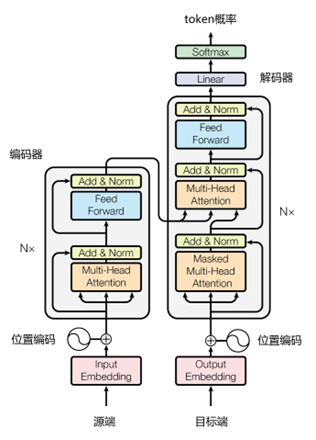
\includegraphics[width=1\textwidth]{figures/Transformer_Structure.png}
	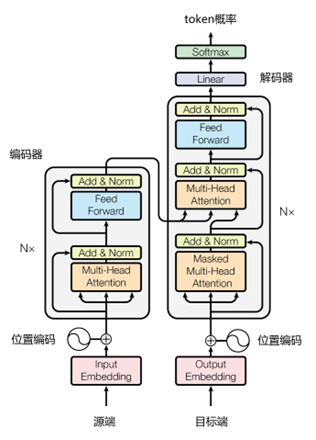
\includegraphics[width=0.8\linewidth]{figures/Transformer_Structure.png}
	\caption{Transformer模型结构\cite{Attn_is_all_you_need}}
	\label{Transformer_Structure}
\end{figure}

\subsection{编码过程}

由于同一个Token在不同位置表达的含义与对整体语义的影响也是不同的,因此只使用Word Embedding表示的信息不够充分,需要引入位置信息,便有了位置编码嵌入(Position Embedding)。本文把Word Embedding与Position Embedding的结合称为输入嵌入(Input Embedding),作为接下来介绍的编码器的输入。

编码器:编码器由$N$个完全相同的层堆叠而成。每一层都有两个子层构成,其中第一个子层是一个多路注意力(Muti-Head Attention,MHA)网络,第二子层是一个简单的、位置完全连接的前馈网络(Feed-Forward Network,FFN)。本文对每个子层进行计算的时候,都先经过一个残差连接层(Residual Connection),接着进行层标准化(Layer Normalization,LN)也就是说,每个子层的输出是LN($x$ + Sublayer($x$)),其中Sublayer($x$)是由子层本身实现的函数。为了保证这些残差连接,模型中的所有子层以及嵌入层产生的输出维度都相同。

注意力机制的基本思路是构建一个映射函数来从一组键-值(Key-Value)对中检索出和给定查询(Query)相关的信息,其中查询、键和值都用向量表示。而注意力网络的输出则为值的加权求和,其中分配给每个值的权重由查询与相应键的兼容性函数计算所得。在Transformer模型中使用了一种特殊的注意力网络结构,称为缩放点积注意力(Scaled Dot-Product Attention)网络。假设输入的查询$Q$和键$K$的维度为$d$,值$V$的维度为$d$,那么注意力网络的整个过程是先计算查询$Q$和每个键$K$的点乘操作,并除以$\sqrt{d}$,然后应用Softmax函数计算权重,最终通过加权求和得到最终的输出:
%$$Attention(Q, K, V)=Softmax((Q\cdot K^T) / \sqrt{d})∙V$$
\begin{equation}
		\text{Attention}(Q, K, V)=\text{Softmax}(\frac{Q\cdot K^T}{\sqrt{d}})∙V\notag
\end{equation}

\subsection{解码过程}

编码器输出的结果是解码器输入的一部分,解码器另外的输入是与Input Embedding生成方式相同的Output Embedding。解码器每次输出的是目标端各Token的“动态”Embedding。取最后一个Token的“动态”Embedding,经过一个线性层输出一个大小为词表大小的浮点数数组,记为Logits,它表示模型输出的词表上每一个词作为下一个Token的可能性,通过Softmax函数转换为0至1之间的值以表征概率,选择概率最大值所对应的下标index来作为输出,这里的下标值是与词表对应的非负整数,其可以通过Tokenzier解码为具体的字符。下面介绍解码器的构成。

解码器:解码器同样由$N$个完全相同的层堆叠而成。除了编码器中用到的两个子层之外,解码器还插入了第三个子层,该层对编码器的输出结果执行多路注意力机制,从而来获取代表源语言端的上下文的向量表示。与编码器类似,Transformer在每个子层先采用残差连接层,然后进行层标准化。由于解码器需要去拟合一个条件语言模型,因此需要在解码器的多路注意力子层中添加一个掩码,以防止每个目标言端的词会直接用到其后面位置的词语信息。这种掩码将输出嵌入偏移一个位置,确保对位置为$i$的词的概率预测只能依赖位置小于$i$的已知输出。

解码器每次输出一个Token,当检测到输出为词表上表示结束的符号“<EOS>”对应的数值时,解码器停止流程,意味着当前解码任务完成,将上面所有解码出来的整数数组通过Tokenizer进行解码,即根据词表从数字映射到字符,便得到了最终的文本输出。

\section{语言模型的记忆问题}

随着深度学习技术的迅速发展,大型语言模型在自然语言处理领域取得了重要突破。例如,GPT系列\cite{GPT2, GPT3}和BERT\cite{BERT}模型已经在多个任务上取得了超越人类的表现。然而,随着模型规模的扩大,其在学习过程中对训练数据的记忆问题引起了关注。研究表明\cite{Extrac_Train_Data_From_LM},这些语言模型可能会在生成结果中泄露训练数据中的敏感信息。下面给出LM记忆问题的定义。

\begin{definition}{模型知识抽取:}
	如果存在前缀$c$,使得下面的式子成立,则称字符串$s$是可从LM(即$f_\theta$)中提取的:
	$$s\leftarrow \mathop{argmax}_{s':|s'|=N} f_\theta(s'|c)$$
	\label{Model_Feature_Extraction}
\end{definition}

在这里用$f_\theta (s'|c)$来表示整个序列为$s'$的可能性。由于在大规模的数据集上计算最可能的序列$s$是非常困难的,定义\ref{Model_Feature_Extraction}中的argmax可以用一个适当的抽样策略(例如贪心采样)来替代,该策略反映了模型$f_\theta$在实际应用中生成文本。

\begin{definition}{$k$-清晰记忆:}
	\label{k_clear_mem}
	如果$s$是可以被从LM($f_\theta$)中提取到的,且$s$在训练数据$X$中最多出现$k\geq1$个例子:$|{x\in X: s\subseteq x}|\leq k$,那么一个字符串$s$是$k$-清晰记忆。
\end{definition}

这个定义的关键是“示例”的含义。对于GPT-2,每个完整网页被用作一个训练示例。由于该定义考虑的是包含给定字符串的不同训练示例的数量,而非该字符串出现的总次数,因此一个字符串在同一页中可能出现多次,但仍被视为$k=1$的记忆。

由于LM是概率生成模型,本文遵循之前的工作,并使用一种自然的似然度量——困惑度,来评估 LM“预测”序列中Tokens的好坏程度。具体地说,

\begin{definition}{困惑度(Perplexity):}
	对于一个Tokens序列:$(x_1,\dots,x_n )$,其困惑度的定义如下:
	$$p=\exp(-\frac{1}{n}\sum_{i=1}^{n}\log f_\theta(x_i|(x_1,\dots,x_{i-1}))$$
	\label{PPL}
\end{definition}

上式中的$f_\theta(x_i|(x_1,\dots,x_{i-1})$为在前面$(x_1,\dots,x_{i-1})$这些tokens的语境下,模型$f_\theta$判定下一个Token为指定Token的概率。由于经过\rm{Softmax}输出后的概率$0<p<1$,对其取负对数后变为$0 < -\log p < +\infty$,从前往后对每个Token计算上述结果,并取其均值作为结果。因此,如果困惑度较低,则模型对生成的Token序列不太“惊讶”(即该序列较为连贯),并为序列中每个Token分配了高概率。


\subsection{训练样本推断攻击} \label{训练样本推断攻击-实验设置}

\subsubsection{攻击描述与设置}

本章中的训练样本推断攻击是属于攻击方式中的模型反演攻击。模型反演攻击(Model Inversion Attack)是针对机器学习模型的一种隐私攻击方法。在这种攻击中,攻击者试图通过已知的模型输出(预测结果)以及对模型的访问权限,推断出输入数据的某些敏感特征。该攻击方法侧重于特定个体的敏感信息泄露问题。

模型反演攻击通常分为白盒和黑盒两种场景。在黑盒攻击中,攻击者仅具有有限的模型访问权限,例如仅能使用模型的预测API。攻击者可以通过探测模型的输入-输出关系,以便从模型的预测结果中提取特定用户的敏感信息。黑盒攻击通常需要攻击者具备一定的辅助信息(如输入数据的部分特征或标签信息),以便构建输入并分析输出。在白盒攻击中,攻击者可以直接访问模型的内部结构、权重和参数。这使得攻击者能够更深入地了解模型的工作原理,并更容易地提取输入数据的敏感信息。白盒攻击通常具有更高的成功率,但在实际场景中,攻击者通常很难获得模型的完整访问权限。

模型反演攻击的成因主要是模型在训练过程中学到了输入数据的某些敏感特征。这些特征可能会用于生成预测结果,从而使攻击者有机会从输出中提取这些特征。

本实验假设恶意攻击者对模型执行黑盒攻击,即攻击者只能从输入与模型的输出关系来推测隐私信息。

\subsubsection{实验设置}

这里的实验环境如表\ref{chap3_exp1_env}所示:CPU为AMD Ryzen 9 5900HX、32GB RAM、GPU为RTX3080-Laptop、操作系统为Windows 11 64位。

\begin{table}[]
	\centering
	\caption{实验环境}
	\begin{tabular}{|c|c|}
		\hline
		维度&配置
		\\ \hline
		
		处理器&AMD Ryzen 9 5900HX @ 3.30GHz    \\ \hline
		内存&32G DDR4 3200Hz    \\ \hline
		GPU&RTX3080-Laptop 16G VRAM    \\ \hline
		操作系统&Windows 11 64位    \\ \hline
		硬盘&1TB SSD    \\ \hline
	\end{tabular}
	\label{chap3_exp1_env}
\end{table}

%本节使用的LM是Hugging Face中的一个中文GPT2模型\footnote{https://huggingface.co/uer/gpt2-chinese-cluecorpussmall},其参数量为81.9M,使用的词表大小为21128,隐层维度为768,使用12层的GPT2Block,其结构如图\ref{GPT2-small}所示。其中wte表示Word Token Embedding,,它的维度为(词表大小,隐层维度),即为词表上所有tokens的768维的嵌入表示。另一个初始Embedding,即wpe表示Word Position Embedding,它表示token的位置编码,维度为(最大长度,隐层维度),这里为1024,表示该语言模型支持最多1024各token作为输入。在编码过程中,由Token Embedding与Position Embedding组合而成的维度为(token长度,768)的Input Embedding通过12层GPT2Block,得到每个token的最终Embedding。为了输出下一个token,最后一个token的最终Embedding在通过最后的lm\_head,将768维的隐层表示映射到词表大小上,以表示语言模型认为词表上每一个token作为下一个token的置信度。

本节使用的LM是Hugging Face中的一个中文GPT2模型\footnote{https://huggingface.co/uer/gpt2-chinese-cluecorpussmall},其参数量为81.9M,使用的词表大小为21128,隐层维度为768。模型由12层GPT2Block组成,其结构如图\ref{GPT2-small}所示。其中,wte表示Word Token Embedding,维度为(词表大小,隐层维度),即为词表上所有Tokens的768维嵌入表示。另一个初始Embedding,即wpe表示Word Position Embedding,它表示Token的位置编码,维度为(最大长度,隐层维度),这里为1024,表示该语言模型支持最多1024个Token作为输入。在编码过程中,由Token Embedding与Position Embedding组合而成的维度为(句子Tokens长度,768)的Input Embedding通过12层GPT2Block,得到每个Token的最终Embedding。为了输出下一个Token,最后一个Token的最终Embedding在通过最后的lm\_head,将768维的隐层表示映射到词表大小上,以表示语言模型认为词表上每一个Token作为下一个Token的置信度。

\begin{figure}[h]
	\centering
	%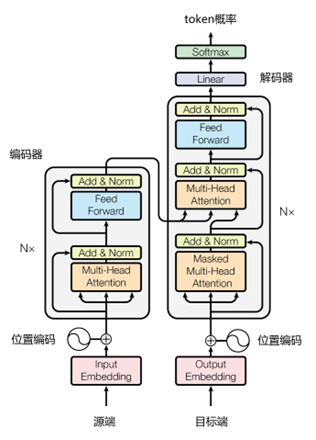
\includegraphics[width=1\textwidth]{figures/Transformer_Structure.png}
	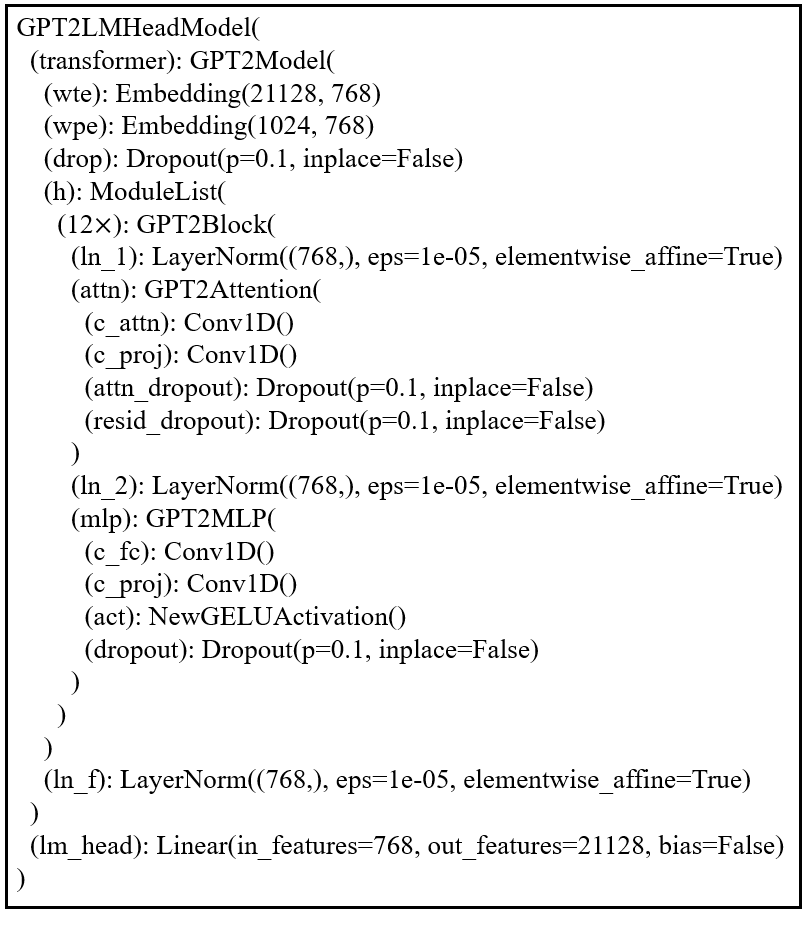
\includegraphics[width=0.7\linewidth]{figures/GPT2_Structure.png}
	\caption{使用中文词表的GPT2-small模型}
	\label{GPT2-small}
\end{figure}

\subsubsection{攻击结果}

%使用该预训练模型进行解码时,超参数设定如下:温度$T=0.5$,$top_k=20$,$repitition_penalty=5$。当传入的前缀$prefix$=“我的手机号是156”时,采用上述攻击方式得到的部分结果如图\ref{AttackLMPrefixIS156}所示的解码结果。

本节使用该预训练模型进行解码,其超参数设置如下:温度T=0.5,top\_k=20,repitition\_penalty=5。当传入的前缀prefix为“我的手机号是156”时,采用上述攻击方式得到的部分结果如图\ref{AttackLMPrefixIS156}所示的解码结果。


\begin{figure}[h]
	\centering
	%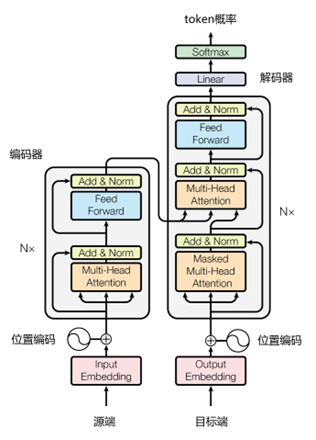
\includegraphics[width=1\textwidth]{figures/Transformer_Structure.png}
	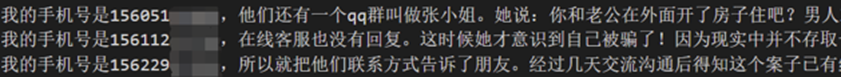
\includegraphics[width=\linewidth]{figures/AttackLMPrefixIS156.png}
	\caption{针对公开语言模型攻击的结果}
	\label{AttackLMPrefixIS156}
\end{figure}

下面验证攻击结果的准确性。由于LM生成的结果可能包含随机生成的结果。随后使LM生成若干条结果对生成的结果进行筛选,过滤掉其中不符合手机号长度与字符的生成样本,剩下的即为可能的攻击结果。为了检验生成结果的正确性,第一种验证方式是通过微信添加好友输入生成的结果,若可以检索到用户则为成功,这也是最为强力的验证手段;第二种方式是通过如百度、谷歌等各种搜索引擎检索,若有部分符合区域的前7位段号,则也认为该生成结果是成功的。图\ref{AttackWeChatRes}为恢复出结果并检验成功的部分样例,具体情况如表\ref{Prefix_Attack_Table}所示。

本节中的攻击方式为黑盒攻击,即攻击者只能从输入与模型的输出关系中推测隐私信息。在解码时,本节使用预训练模型生成多条结果,并从中过滤掉其中不符合手机号长度与字符的生成样本,剩余的生成结果为可能的攻击结果。本节使用两种方式验证生成结果的准确性:第一种是通过微信添加好友输入生成结果,若可以检索到用户则为成功;第二种是通过搜索引擎(如百度、谷歌等)检索,若有部分符合区域的前7位段号,则也认为该生成结果是成功的。图\ref{AttackWeChatRes}展示了成功恢复结果并验证的部分样例,具体情况如表\ref{Prefix_Attack_Table}所示。

\begin{figure}[h]
	\centering
	%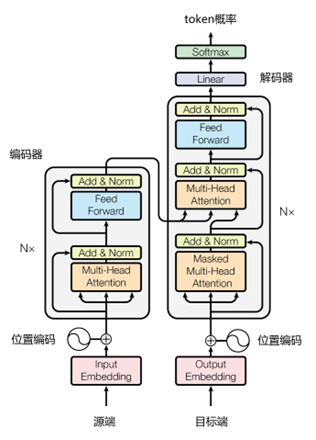
\includegraphics[width=1\textwidth]{figures/Transformer_Structure.png}
	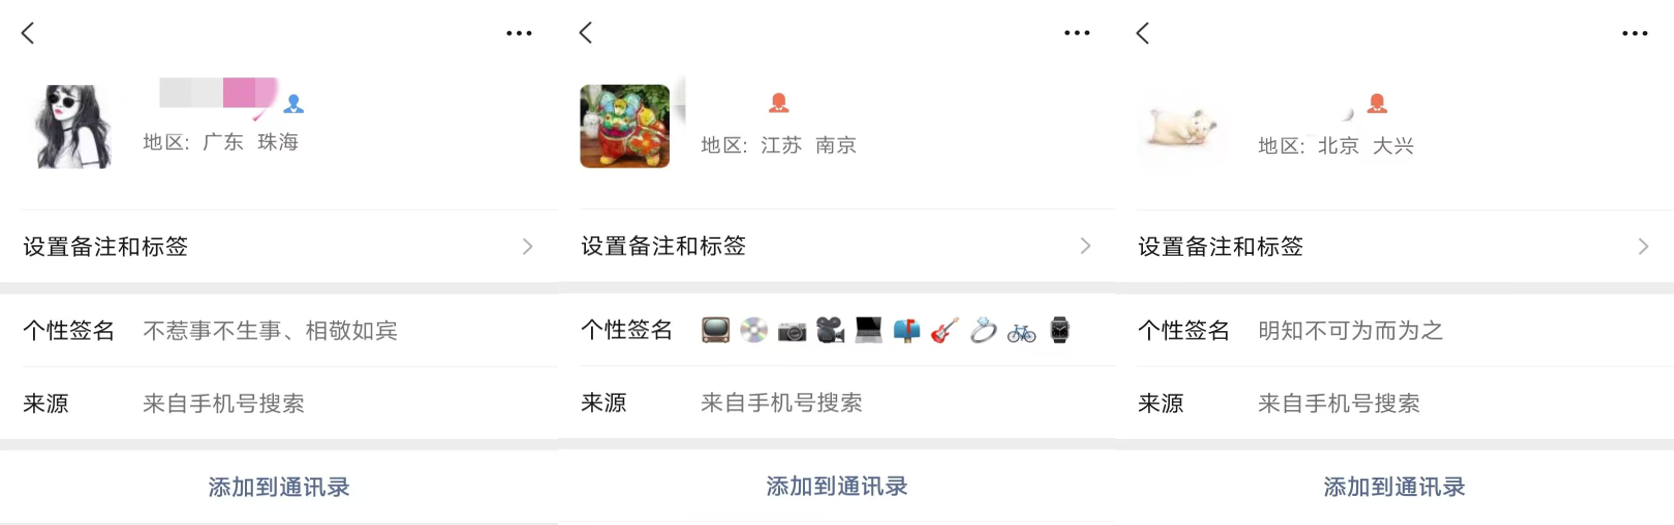
\includegraphics[width=\linewidth]{figures/AttackWeChatRes.png}
	\caption{检验攻击结果的正确性}
	\label{AttackWeChatRes}
\end{figure}

\begin{table}[]
	\centering
	\caption{前缀攻击结果}
	\begin{tabular}{|c|c|c|c|}
		\hline
		总数&不合规&无效&有效   \\ \hline
		100&47&24&29    \\ \hline
	\end{tabular}
	\label{Prefix_Attack_Table}
\end{table}

%该预训练模型公布于2020年,其使用的公开训练数据为:包含19年中文维基百科、16年的新闻预料、18年百科问答等的\footnote{https://github.com/brightmart/nlp\_chinese\_corpus}以及包含2005-2011年间的74万篇新闻文档的\footnote{http://thuctc.thunlp.org/\#中文文本分类数据集THUCNews}等训练语料。由于该LM训练语料较早,其中使用到的隐私信息部分可能处于老旧不可用状态,因此持有更多最新隐私信息的数据持有方训练的模型会面临着更大的隐私问题。

该预训练模型公布于2020年,使用的公开训练数据包含了2019年中文维基百科、2016年的新闻预料、2018年百科问答等\footnote{https://github.com/brightmart/nlp\_chinese\_corpus}以及包含2005-2011年间的74万篇新闻文档的数据集\footnote{http://thuctc.thunlp.org/\#中文文本分类数据集THUCNews}。然而,由于该LM训练语料较早,其中使用到的部分隐私信息可能已过时或不再适用。从本实验结果可以合理推测,使用较新的隐私数据训练的模型可能会面临更大的隐私问题。值得注意的是,此类攻击不仅对公开的预训练模型构成威胁,也会对任何基于语言模型的应用系统产生影响。

\subsection{改进的攻击策略}

\subsubsection{改进的解码方式}

通过过滤低概率样本进行成员推断,由于以下类型语言模型的问题,导致其精度较差:许多样本被分配了虚假的高概率。这类样本主要有两种:

\textbf{琐碎的记忆。}在很多情况下,GPT-2输出的内容是无意义的,因为文本非常常见。例如,它以高概率重复从1到100的数字。

\textbf{重复的子字符串。}LM经常犯的错误是它们倾向于反复生成相同的字符串。很多没有被记忆的高概率样本确实是重复的文本(例如,“我在吃饭。我在吃饭。我在吃饭。……”)。

一个直观的改进想法是通过与第二个LM进行比较,过滤掉这些重复(但仍然是高概率的样本)。假设有第二个模型能够准确捕捉文本的置信度,那么它也会给这些记忆内容赋予高置信度。因此,寻找更多样化、更罕见的记忆形式的一个自然策略是,与第二个模型相比,过滤原始模型的置信度“出乎意料地高”的样本。下面本部分将讨论实现这一目标的四种方法。

(1)与其他LM比较。假设有第二个LM,它记忆的是与原LM不同的一组例子。实现这一目标的一个方法是在一组与GPT-2训练数据不相交的数据上训练模型,这种情况下两个模型记住相同的k-清晰记忆概率较小。另一种策略是采取一个小得多的模型在相同的数据集上训练:因为小模型没有较强的记忆能力。因此本部分假设,存在k-清晰记忆的样本,使得其被大规模的LM模型记住,但不被小LM模型记住。

(2)与zlib压缩比较。实验中不必与另一个LM进行比较。对于给定的序列,任何能赋予序列某种感知程度概念的技术都是有用的。作为一种简单的基线方法,本部分计算文本的zlib熵\cite{zlib}:序列用zlib压缩时的熵位数。然后,本部分使用原LM困惑度和zlib熵的比值作为本部分的成员推断度量。虽然文本压缩器很简单,但它们可以识别出上面描述的无意义的重复例子(例如,它们在建模重复子字符串方面非常出色)。

(3)滑动窗口的困惑度。有时,当样本包含一个记忆的子字符串,周围是一块非记忆(和高困惑度)的文本时,模型给出的置信度不高。为了处理这个问题,本部分取以特定长度Tokens为滑动窗口的最小的困惑度作为结果。

(4)基于衰减温度的采样。如\ref{NLP_Def}节所述,给定之前的Tokens序列,LM产生下一个Token的概率:$Pr(x_i |x_1,⋯,x_{i-1} )$。在实践中,这是通过神经网络$f_θ(x_i|x_1,⋯,x_{i-1})$来得到“logit”向量$z$,然后计算Softmax$(z)$得到输出概率分布。

对于$t>1$,可以通过将输出Softmax$(z)$替换为Softmax$(\frac{z}{t})$来人为地“压平”这个概率分布,使模型输出的置信度差距不会太大(这里,$t$被称为温度)。即温度越高,模型的输出越多样化。

然而,在整个生成过程中保持较高的温度意味着,即使采样过程开始发出一个记忆的例子,它也可能会随机偏离记忆输出的路径。因此,使用一种动态衰减的温度可以为模型提供了足够的时间来“探索”一组不同的前缀,同时也允许它遵循它找到的高置信路径。

%一个直观的想法是通过与第二个LM进行比较,过滤掉这些重复(但仍然是高可能性的样本)。假设有第二个模型能够准确捕捉文本的置信度,那么它也会这些记忆内容给出高置信度。因此,寻找更多样化、更罕见的记忆形式的一个自然策略是,与第二个模型相比,过滤原始模型的置信度“出乎意料地高”的样本。下面我们将讨论实现这一目标的四种方法。
%
%
%(1)与其他LM比较。假设我们有第二个LM,它记忆的是与原LM不同的一组例子。实现这一目标的一个方法是在一组与GPT-2训练数据不相交的数据上训练模型,在这种情况下两个模型将记住相同的k-清晰记忆不太可能。另一种策略是采取一个小得多的模型在相同的数据集上训练:因为小模型没有较强的记忆能力。我们猜想,存在k-清晰记忆的样本,使得其被大规模的LM模型记住,但不被小LM模型记住。
%
%(2)与zlib压缩比较。 我们不必与另一个LM进行比较。对于给定的序列,任何能赋予序列某种感知程度概念的技术都是有用的。作为一种简单的基线方法,我们计算文本的zlib熵\cite{zlib}:序列用zlib压缩时的熵位数。然后,我们使用原LM困惑度和zlib熵的比值作为我们的成员推断度量。虽然文本压缩器很简单,但它们可以识别出上面描述的平凡的记住的信息和重复的例子(例如,它们在建模重复子字符串方面非常出色)。
%
%(3)滑动窗口的困惑度。 有时,当样本包含一个记忆的子字符串,周围是一块非记忆(和高困惑度)的文本时,模型给出的置信度不高。为了处理这个问题,我们取以特定长度tokens为滑动窗口的最小的困惑度作为结果。
%
%(4)基于衰减温度的采样。 如\ref{NLP_Def}节所述,给定之前的tokens序列,LM产生下一个token的概率:$Pr(x_i |x_1,⋯,x_{i-1} )$。在实践中,这是通过神经网络$f_θ(x_i|x_1,⋯,x_{i-1})$来得到“logit”向量$z$,然后计算$\rm{Softmax}(z)$得到输出概率分布。
%
%对于$t>1$,可以通过将输出$\rm{Softmax}(z)$替换为$\rm{Softmax}(\frac{z}{t})$来人为地“压平”这个概率分布,使模型输出的置信度差距不会太大(这里,$t$被称为温度)。即温度越高,模型的输出越多样化。
%
%然而,在整个生成过程中保持较高的温度意味着,即使采样过程开始发出一个记忆的例子,它也可能会随机偏离记忆输出的路径。因此,使用一种动态衰减的温度可以为模型提供了足够的时间来“探索”一组不同的前缀,同时也允许它遵循它找到的高置信路径。


\subsubsection{攻击结果} \label{Chap3_meminfer_setting}

这里实验环境与\ref{训练样本推断攻击-实验设置}相同:CPU为AMD Ryzen 9 5900HX、32GB RAM、GPU为RTX3080-Laptop、操作系统为Windows 11 64位。

实验结果如表\ref{Remaster_Attack_Method_with_Num_Success}所示。其中另一个LM选择的是原始的GPT2模型\cite{GPT2}(主要的训练语料是英文),在使用滑动窗口的困惑度解码时滑动窗口的大小设置为3;使用温度衰减时从$t=10$开始,在前8个Tokens内线性衰减到$t=1$(由于最关注的输出部分是一开始的11位手机号156XXXXXXXX,需要8位输出),之后保持$t=1$。

\begin{table}[]
	\centering
	\caption{改进的前缀攻击结果}
	\begin{tabular}{|c|c|c|c|}
		\hline
		方式&不合规&无效&有效   \\ \hline
		原始生成&43&28&29    \\ \hline
		与其他LM比较&39&32&29    \\ \hline
		与Zlib压缩比较&41&31&28    \\ \hline
		使用滑动窗口&36&38&26    \\ \hline
		使用温度衰减&44&32&24    \\ \hline
	\end{tabular}
	\label{Remaster_Attack_Method_with_Num_Success}
\end{table}

%从表\ref{Remaster_Attack_Method_with_Num_Success}可以看出,虽然上述改进的攻击方式的有效比例跟原始的直接生成差别不大,但是从合规的角度,即满足输出的位数是11位手机号的形式,这些攻击方式基本都比原始生成要好,这也证明了这些攻击方式可以生成更符合预期推断目的的生成结果。此外,由于人工验证的开销太大,无法执行更大规模的验证,只使用“156”作为开头以及仅100条记录的生成结果可能包含很多随机性。

从表\ref{Remaster_Attack_Method_with_Num_Success}可以看出,虽然上述改进的攻击方式的有效比例跟原始的直接生成差别不大,但是从合规的角度,即满足输出的位数是11位手机号的形式,这些攻击方式基本都比原始生成要好,这也证明了这些攻击方式可以生成更符合预期推断目的的生成结果。此外,由于人工验证的开销太大,无法执行更大规模的验证,只使用“156”作为开头以及仅100条记录的生成结果可能包含很多随机性。


%\section{面向攻击者在训练阶段试图推断隐私数据以及破坏训练协议的攻击}
\section{训练阶段推断隐私数据以及破坏训练协议的攻击}

%===恶意场景,跟相关工作定义恶意相同,1.分析半诚实模型在恶意情况失效的原因2.单纯把用可信执行环境当作可信第三方的问题;;;理论分析跟实际实验一致===

\subsection{场景描述与安全假设}

%===恶意攻击者的描述,其可以执行xxx等侧信道攻击===

%在这种场景下,我们假设有两类实体,一方是多个拥有医疗隐私数据的数据持有者,另一方是提供计算服务的多个计算方。多个数据持有者希望通过多个计算方提供的计算服务来协同训练模型,计算方在计算服务结束后将训练好的模型分发给各个数据持有者。
%
%与该场景下的常见假设相同\cite{SecureNN, SecureNLP},本文对该场景下数据持有者的安全假设是其会严格遵循协议提供本地数据并且不会推测其他数据持有者的隐私数据,即数据持有者是诚实的。对计算方的安全假设是其可以任意偏离协议并且会从获取到的数据推断数据持有者的隐私信息以及模型参数,即计算方是恶意的。与相关研究\cite{Cryptflow}的设定相同,这种恶意假设是合理且常见的。此外,本文假设多个恶意计算方不会共谋。

在这种场景下,本节假设存在两类实体,一方是拥有医疗隐私数据的多个数据持有者,另一方是提供计算服务的多个计算方。这些数据持有者希望利用计算方提供的服务,协同训练一个模型。计算方在计算服务结束后,将训练好的模型分发给各个数据持有者。

本文遵循常见的安全假设\cite{SecureNN, SecureNLP},认为数据持有者会严格遵循协议提供本地数据,且不会试图推断其他数据持有者的隐私数据,即数据持有者是诚实的。对于计算方,本部分假设它们可能会任意偏离协议,试图从获取的数据中推断数据持有者的隐私信息以及模型参数,即计算方是恶意的。与相关研究\cite{Cryptflow}的设定相同,这种恶意假设是合理且常见的。此外,本文假设多个恶意计算方不会共谋。

\subsection{攻击方式与攻击效果}

本部分从两个方向展开分析。首先,本部分讨论针对基于多方计算(MPC)的当前工作所面临的问题;其次,本部分分析引入可信执行环境的相关工作面临的攻击。

当前针对机器学习与深度学习领域的基于MPC的相关工作(如SecureNN\cite{SecureNN}、SecureNLP\cite{SecureNLP}和ABY3\cite{aby3}等)可以在半诚实攻击者的安全假设下保障协议的安全性。然而,面对恶意攻击者,不仅可能根据获取到的内容推断更多信息,还可能在执行过程中任意偏离协议,即返回任意非正常结果\cite{Cryptflow}。这意味着在执行过程中,恶意攻击者负责的计算部分可能会遭受破坏,从而导致整个协议的执行过程受到破坏。

为了规范计算方的行为,部分研究集中于使用硬件设备来保护数据隐私以及执行过程的安全。例如,Lee等人\cite{lee2019occlumency}提出了一种名为Occlumency的创新性云驱动解决方案,旨在在不影响使用强大云资源优势的前提下,保护用户隐私。Occlumency利用SGX的Enclave在整个深度学习推理过程中保护用户数据的机密性和完整性。Hua等人\cite{hua2020guardnn}提出了一种名为GuardNN的安全深度神经网络加速器,它在不受信任的环境中为用户数据和模型参数提供基于硬件的保护。作者通过针对已知的DNN加速器内存访问模式定制片外存储器保护,将内存加密和完整性验证的开销降至最低,并在可编程门阵列上进行了原型实现,验证了该方案对推理任务提供了有效的保密性保护。Hashemi等人\cite{hashemi2020darknight}提供了一个统一的大型深度神经网络的训练和推理框架,旨在在保护输入隐私和计算完整性的同时进行训练和推理。作者提出了一种名为DarKnight的方法,它使用一种基于矩阵掩蔽的新颖数据盲化策略,在可信执行环境中创建输入混淆。并通过分析证明了其信息论隐私保证。

尽管上述工作都将可信硬件Intel SGX视为一个可信第三方,即其可以提供机密性与完整性,但自Intel推出SGX以来,各种攻击接踵而至。其中最具代表性的攻击是侧信道攻击,如功耗分析攻击、计时攻击、回滚攻击与缓存冲突攻击等\cite{SGX_Exposure, High_Resolution_Side_Channels, Cache_Attack_SGX, CacheZoom, SGX_Cache, mem_side_hazard, PMFaultFA, VoltJockeyAN}。这些攻击通常会攻破可信硬件,从而破坏其机密性与完整性。

%这里我们从两个方向的分析展开。第一是当前针对该场景下基于MPC的工作所面临的问题,第二是引入可信执行环境的相关工作面临的攻击。
%
%当前针对机器学习与深度学习学习领域下的基于MPC的相关工作\cite{SecureNN, SecureNLP, aby3}等工作可以在半诚实攻击者的安全假设下保障协议的安全性。而常见的针对恶意攻击者的假设是其不仅可以根据获取到的内容来推断更多的信息,而且在执行过程中可以任意偏离协议,即其可以返回任意非正常结果\cite{Cryptflow}。这样在执行过程中恶意攻击者负责的计算部分就会面临着恶意攻击者的破坏,从而导致整个协议的执行过程遭到破坏。
%
%为规范计算方的行为,部分工作聚焦到使用硬件设备来保护数据隐私以及执行过程的安全,如Lee等人\cite{lee2019occlumency}提出了一种名为Occlumency的创新性云驱动解决方案,旨在在不影响使用强大云资源优势的前提下,保护用户隐私。Occlumency利用SGX的Encalve来在整个深度学习推理过程中保护用户数据的机密性和完整性。Hua等人\cite{hua2020guardnn}提出了一种名为GuardNN的安全深度神经网络加速器,它在不受信任的环境中为用户数据和模型参数提供基于硬件的保护。作者通过针对已知的DNN加速器内存访问模式定制片外存储器保护,将内存加密和完整性验证的开销降至最低,并在可编程门阵列上进行了原型实现,验证了该方案对推理任务提供了有效的保密性保护。Hashemi等人\cite{hashemi2020darknight}提供了一个统一的大型深度神经网络的训练和推理框架,旨在在保护输入隐私和计算完整性的同时进行训练和推理。作者提出了一种名为DarKnight的方法,它使用一种基于矩阵掩蔽的新颖数据盲化策略,在可信执行环境中创建输入混淆。并通过分析证明了其信息论隐私保证。
%
%上述针对工作均将可信硬件Intel SGX视为一个可信第三方,即其可以提供机密性与完整性。然而,自Intel推出SGX以来,各种攻击接踵而至。其中最具有代表性的攻击时侧信道攻击,如功耗分析攻击、计时攻击、回滚攻击与缓存冲突攻击等\cite{SGX_Exposure, High_Resolution_Side_Channels, Cache_Attack_SGX, CacheZoom, SGX_Cache, mem_side_hazard, PMFaultFA, VoltJockeyAN}。这些攻击通常会攻破可信硬件,从而破坏其机密性与完整性。



\section{推断阶段恢复训练隐私数据的攻击}\label{chap3_CMDD_FT_Exp}

%本节我们通过对由原始训练数据训练得到的模型执行模型反演攻击,结果表明模型可以记住训练数据隐私信息。
本节通过对由原始训练数据训练得到的模型执行模型反演攻击,结果表明模型可能记忆训练数据隐私信息。

%首先,本部分通过实验来说明在中文医学场景下,LM的记忆性问题依然很突出,即从公开的预训练模型来尝试生成训练样本并验证成功率。其次,在医学文本生成任务场景下,本节在公开预训练模型的基础上,通过医学文本数据集来微调LM,并测试针对训练好的模型的训练数据重构攻击的攻击效果。最后,本节对攻击策略进行改进,并通过实验说明这些改进可以从LM中抽取更多的隐私训练数据。

首先,本部分通过实验来说明在中文医学场景下,语言模型的记忆性问题依然突出,即尝试从公开预训练模型生成训练样本并验证成功率。其次,在医学文本生成任务场景下,本节在公开预训练模型基础上通过医学文本数据集微调语言模型,测试针对训练好的模型的训练数据重构攻击效果。最后,本节对攻击策略进行改进,并通过实验说明这些改进可以从语言模型中抽取更多隐私训练数据。

\subsection{场景描述与安全假设}

%在这种场景下,我们假设有两类实体,一方是模型的持有者,另一方是使用模型推断服务的使用方。本文对该场景下的模型持有者的安全假设是其会严格遵循协议执行推断过程,对使用方的假设是其可以通过模型推断服务执行输入和标签重构攻击等攻击方式来恢复模型的训练隐私数据,即模型持有者是诚实的,而使用方是恶意的。

在这种场景下,本部分假设有两类实体,一方是模型持有者,另一方是使用模型推断服务的使用方。本文假设模型持有者严格遵循协议执行推断过程,对使用方的假设是其可通过模型推断服务执行输入和标签重构攻击等手段恢复模型训练隐私数据,即模型持有者是诚实的,而使用方是恶意的。

\subsection{攻击方式与攻击效果}

%与\ref{训练样本推断攻击-实验设置}节的设定相同,本部分考虑针对模型输出结果的恢复训练隐私数据的攻击,即执行模型反演攻击。本章考虑攻击者的访问权限是黑盒访问权限。

与\ref{训练样本推断攻击-实验设置}节设定相同,本部分考虑针对模型输出结果的恢复训练隐私数据攻击,即执行模型反演攻击。本章考虑攻击者的访问权限是黑盒访问权限。

\subsubsection{实验设置} \label{chap3_exp_setting}


%目前可以访问到的医学场景下的数据集主要是用于计算机视觉处理的图像数据,文本形式的中文数据集很少,而且主要是基于命名实体识别与知识图谱的分类打分等数据,用于生成文本训练并不合适。本文是关于中文医学文本生成的,故需要中文医学相关的对话、总结或者诊断数据集。因此,本文选择中文医疗对话数据集(Chinese medical dialogue data,CMDD)\footnote{https://github.com/Toyhom/Chinese-medical-dialogue-data},它包含了男科、内科、妇产科、肿瘤科、儿科与外科这六个部门的问答句对,如图\ref{CMDD_Data}所示。

本节选择中文医疗对话数据集(Chinese medical dialogue data,CMDD)\footnote{https://github.com/Toyhom/Chinese-medical-dialogue-data},包含六个部门的问答句对,如图\ref{CMDD_Data}所示。

\begin{figure}[h]
	\centering
	%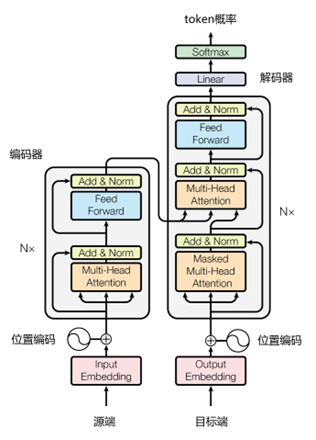
\includegraphics[width=1\textwidth]{figures/Transformer_Structure.png}
	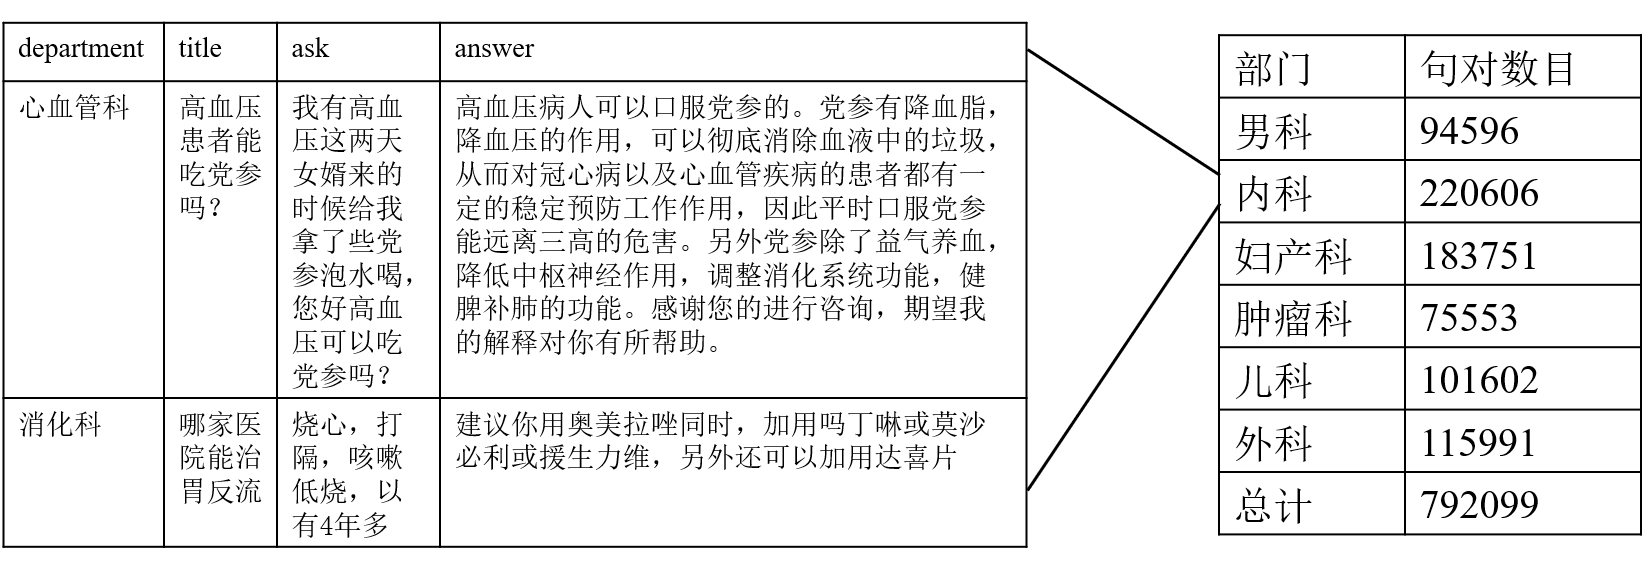
\includegraphics[width=\linewidth]{figures/CMDD_Data.png}
	\caption{CMDD数据集}
	\label{CMDD_Data}
\end{figure}

%为了

%由于该数据集语料较少,而以GPT2-small参数量级别的模型需要的训练语料是千万级别的,而且训练的时间与成本很高。因此,本节是以\ref{训练样本推断攻击-实验设置}节中的中文预训练模型为基础,在上述CMDD数据集上进行微调训练的。

本节以\ref{训练样本推断攻击-实验设置}节中的中文预训练模型为基础,在CMDD数据集上进行微调训练。实验环境与\ref{训练样本推断攻击-实验设置}相同。

这里实验环境与\ref{训练样本推断攻击-实验设置}相同:CPU为AMD Ryzen 9 5900HX、32GB RAM、GPU为RTX3080-Laptop、操作系统为Windows 11 64位。

本节复用了\ref{训练样本推断攻击-实验设置}节中公开语言模型的词表与模型结构,使用的超参数:训练轮数epochs=25,warmup\_steps=1000,学习率为$1e-6$,累积梯度gradient\_accumulation=24,最大梯度裁剪max\_grad\_norm=3。训练过程中使用AdamW优化器,并且使用get\_linear\_schedule\_with\_warmup的设置。


\subsubsection{攻击结果}

(1)正常的生成攻击

%实验过程中的各个Step(模型每通过一个Batch的数据训练更新完称为一个Step)的训练交叉熵Loss与推断的交叉熵Loss均通过TensorBoard的SummaryWriter\cite{tensorflow}记录。训练过程的Loss与Steps之间的关系如图\ref{Chap3_train_loss}所示。从整体来看,训练过程中的Loss并没有减少很多,但是很震荡,原因如下:

实验过程中的每个步骤(模型每通过一个批次的数据训练更新完称为一个步骤)的训练交叉熵损失与推断的交叉熵损失都通过 TensorBoard 的 SummaryWriter\cite{tensorflow} 进行记录。训练过程中的损失值与步骤之间的关系如图 \ref{Chap3_train_loss} 所示。从整体来看,训练过程中的损失在开始的 100k 个步骤时下降较明显,但后面变化不大,整体损失下降的幅度并不大($2.7\rightarrow 1.8$)。同时,损失值的波动较大,原因如下:

\begin{itemize}
	\item [1)]
	损失下降不多。原始的预训练模型是通过大量各种领域的语料训练收敛的,因此在所有中文语义场景的表达已经有了较好的结果,即在 CMDD 医学对话场景下效果也很好。
	\item [2)]
	损失值震荡。由于原始的预训练模型的训练集没有包含很多专门的医学场景语料,因此在医学场景下,如专业名词出现频率低、描述方式较正式、反馈方式独特等特点,模型在某些特殊场景下预测下一个 Token 时可能与实际偏差很大,即 label Token 的概率很低而损失很大。但是大部分对话的逻辑与预训练模型训练过的模式很接近,即大部分预测的比较好。综上所述,在该特定的医学领域对预训练模型进行微调时,损失值的震荡现象属于正常现象。
\end{itemize}

\begin{figure}[h]
	\centering
	%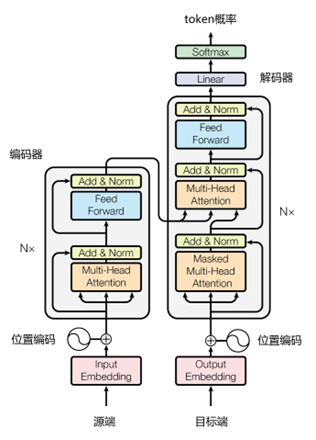
\includegraphics[width=1\textwidth]{figures/Transformer_Structure.png}
	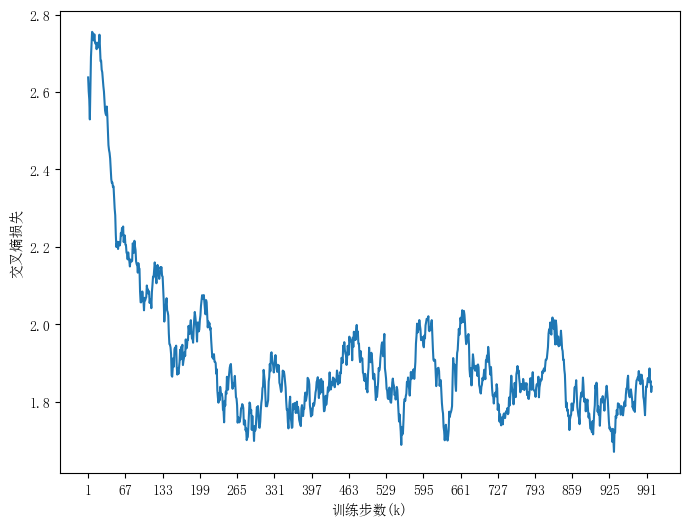
\includegraphics[width=\linewidth]{figures/Chap3_train_loss.png}
	\caption{训练过程中的交叉熵损失与训练步数的关系}
	\label{Chap3_train_loss}
\end{figure}


%不同Epoch下,模型在训练集与验证集上的交叉熵损失函数CrossEntropyLoss如图\ref{CMDD_Train_Valid_Result_Chap3}所示。从图\ref{CMDD_Train_Valid_Result_Chap3}中可以看出,在前15个Epoch中,训练集的Loss在稳步下降,后面趋于平稳,而验证集的Loss在前10个Epoch中稳步下降,后面近乎收敛。在第6个Epoch时,二者数值近似相等,后面模型更倾向于学习到训练集上面数据分布的特点,即训练集的Loss要比验证集Loss要低。从训练过程的损失情况来看,我们采用第10个Epoch的模型参数作为结果来分析语言模型的记忆性。

在不同的 Epoch 下,模型在训练集与验证集上的交叉熵损失函数 CrossEntropyLoss 如图 \ref{CMDD_Train_Valid_Result_Chap3} 所示。从图 \ref{CMDD_Train_Valid_Result_Chap3} 中可以看出,在前 15 个 Epoch 中,训练集的损失值稳步下降,后面趋于平稳;而验证集的损失值在前 10 个 Epoch 中稳步下降,后面近乎收敛。在第 6 个 Epoch 时,二者数值近似相等,之后模型更倾向于学习训练集上的数据分布特点,即训练集的损失值要比验证集的损失值低。从训练过程的损失情况来看,本节采用第 10 个 Epoch 的模型参数作为结果,以分析语言模型的记忆性。

\begin{figure}[h]
	\centering
	%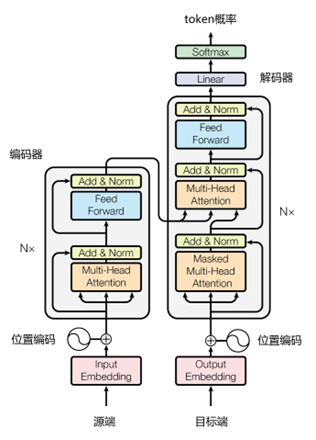
\includegraphics[width=1\textwidth]{figures/Transformer_Structure.png}
	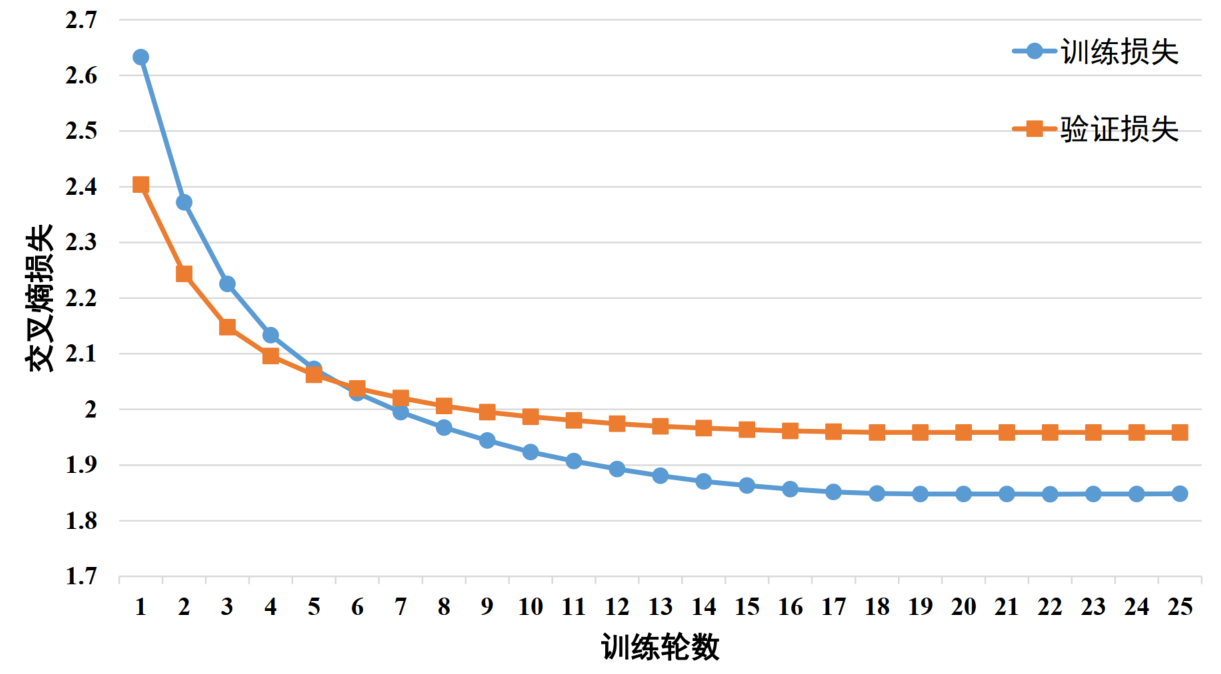
\includegraphics[width=\linewidth]{figures/CMDD_Train_Valid_Result_Chap3.png}
	\caption{使用CMDD数据集微调GPT2-Chinese的Loss随Epoch的变化}
	\label{CMDD_Train_Valid_Result_Chap3}
\end{figure}

(2)改进的生成攻击

%本实验使用随机采样的的10个训练数据的前10个token作为前缀输入,使用\ref{训练样本推断攻击-实验设置}中的方式分别进行解码,测试其完整恢复训练数据的次数。具体来说,对于每个前缀,本节对上述每个前缀生成10000个解码结果,针对其进行平均统计(平均值为分数则向下取整)。

本实验使用随机采样的 10 个训练数据的前 20 个 Token 作为前缀输入,采用\ref{训练样本推断攻击-实验设置}中的方式分别进行解码,测试其完整恢复训练数据的次数。具体来说,对于每个前缀,本节对上述每个前缀生成 10000 个解码结果,针对其进行平均统计(平均值为分数时向下取整)。

%例如,当输入前缀为“我弟弟在的那个补习班”(此为训练数据中出现的样本中的前20个tokens),设置解码长度为20,即让训练的LM生成接下来的20个token。图\ref{Decode_Raw_CMDD_Prefix}为成功恢复出训练样本的一个实例。

例如,当输入前缀为“我弟弟在的那个补习班”(这是训练数据中出现的样本中的前20个Tokens),设置解码长度为20,即让训练的 LM 生成接下来的20个Tokens。图 \ref{Decode_Raw_CMDD_Prefix} 为成功恢复出训练样本的一个实例。

\begin{figure}[h]
	\centering
	%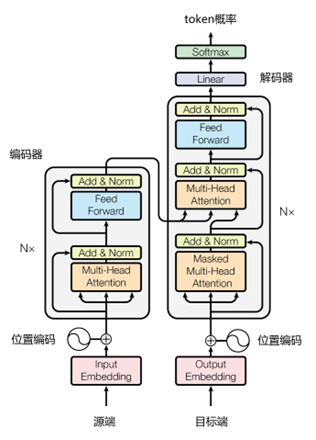
\includegraphics[width=1\textwidth]{figures/Transformer_Structure.png}
	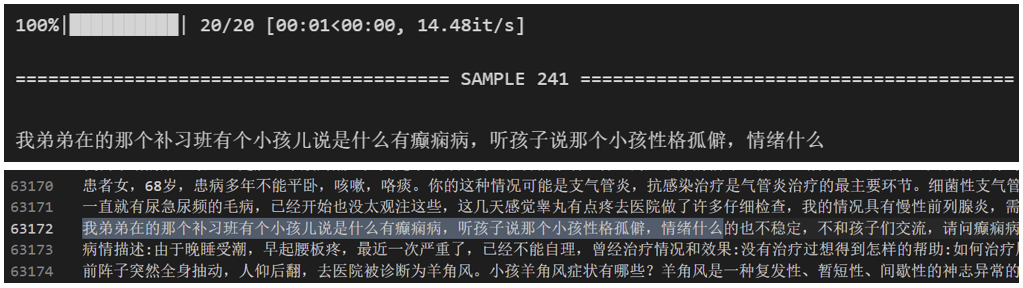
\includegraphics[width=1\linewidth]{figures/Decode_Raw_CMDD_Prefix.png}
	\caption{模型恢复出训练数据中一个样本的前40个Tokens}
	\label{Decode_Raw_CMDD_Prefix}
\end{figure}

%本实验共产生10000个生成样本,过将这10000个生成结果的前20个tokens与原样本的采样后的20个token进行比较,如果全部相同,则成功恢复次数加一。实验结果如表\ref{Attack_Method_with_Num_Success}所示。其中与其他LM比较的另一个LM选择的是原始的GPT2模型\cite{GPT2}(主要的训练语料是英文),使用滑动窗口的困惑度解码中滑动窗口的大小设置为5;使用温度衰减时从$t=10$开始,在前10个tokens的一段时间内衰减到$t=1$(≈序列长度的50\%),之后保持$t=1$。

本实验共产生 10000 个生成样本。将这 10000 个生成结果的前 20 个 Tokens 与原样本的采样后的 20 个 Tokens 进行比较,如果全部相同,则成功恢复次数加一。实验结果如表 \ref{Attack_Method_with_Num_Success} 所示。其中与其他 LM 比较的另一个 LM 选择的是原始的 GPT2 模型\cite{GPT2}(主要的训练语料是英文),使用滑动窗口的困惑度解码时,滑动窗口的大小设置为 5;使用温度衰减时,从 $t=10$ 开始,在前 10 个 Tokens 的一段时间内衰减到 $t=1$ (≈序列长度的 50\%),之后保持 $t=1$。

\begin{table}[]
	\centering
	\caption{攻击方式与成功次数}
	\begin{tabular}{|c|c|}
		\hline
		类型&成功次数   \\ \hline
		原始生成& 14    \\ \hline
		与其他LM比较&19   \\ \hline
		与Zlib压缩比较&14    \\ \hline
		使用滑动窗口&8    \\ \hline
		使用温度衰减&10    \\ \hline
	\end{tabular}
	\label{Attack_Method_with_Num_Success}
\end{table}

上述实验攻击出的成功次数较少,而研究工作\cite{Extrac_Train_Data_From_LM}的文中给出的结果相对而言更多,可能的原因如下:一方面,本实验的LM参数量较少,只有81.9M,而文章\cite{Extrac_Train_Data_From_LM}使用的GPT2-large为1.5B的参数量,更多参数量能够让模型记住更多的信息,这一点在相关文献中得到证实\cite{makingPTLM_few_shot, EmergentLLM, systematicLLM, GPT2, GPT3, BERT};另一方面,本实验的训练语料较少,LM还没充分的学到医学文本生成场景下的特点,导致其困惑度仍较高。

\section{本章小结}

%本章主要探讨了医学文本生成任务在训练和推断阶段的隐私泄露风险,以证明后续提出的隐私保护机制的重要性。首先,我们从语言模型的生成过程出发,详细介绍了如何为自然语言文本建模并生成后续文本,为后续分析医学文本生成模型的训练与推断阶段的执行过程奠定了基础。接着,我们分析了语言模型的记忆问题,并针对公开的预训练模型进行了攻击实验。同时,我们还提出了若干改进的攻击策略以增加攻击效果。此外,本章还讨论了攻击者在训练阶段如何尝试推断隐私数据以及破坏训练协议的可能攻击手段。最后,我们从推断阶段的攻击角度出发,阐述了攻击者可能尝试通过执行输入和标签重构攻击来恢复训练隐私数据的方式。通过在医学文本数据下训练的语言模型攻击实验,我们展示了语言模型记忆问题带来的隐私挑战。

本章探讨医学文本生成任务在训练和推断阶段中的隐私泄露风险,以证明隐私保护机制的必要性。首先,本章详细介绍了语言模型的生成过程,为后续分析医学文本生成模型的训练与推断阶段的执行过程奠定了基础。接着,本章分析了语言模型的记忆问题,并进行了攻击实验及提出改进的攻击策略。同时,本章还探讨了攻击者在训练阶段如何尝试推断隐私数据以及破坏训练协议的可能攻击手段。最后,本章阐述了攻击者可能尝试通过执行输入和标签重构攻击来恢复训练隐私数据。通过在医学文本数据下训练的语言模型攻击实验,本章展示了语言模型记忆问题带来的隐私挑战。本章的内容强调了隐私保护在医学文本生成任务中的重要性。